% Team 8 evidence regenerated by the unified branch. The rolling OOS figure is
% rendered from a frozen aggregate CSV because licensed option bars are local-only.

\subsubsection{Regenerated market-input and return evidence}

The scalar calibration errors reported above are interpretable only together
with the empirical objects that generated them. Figure~\ref{fig:t8-market-inputs}
shows the dated Treasury proxy and the structured option sample rebuilt by the
unified branch from the 2 September 2026 Team 8 snapshot. The raw licensed rows
remain local and Git-ignored; the figures and aggregate calibration outputs
carry hashes in the code-run manifest.

\begin{figure}[H]
    \centering
    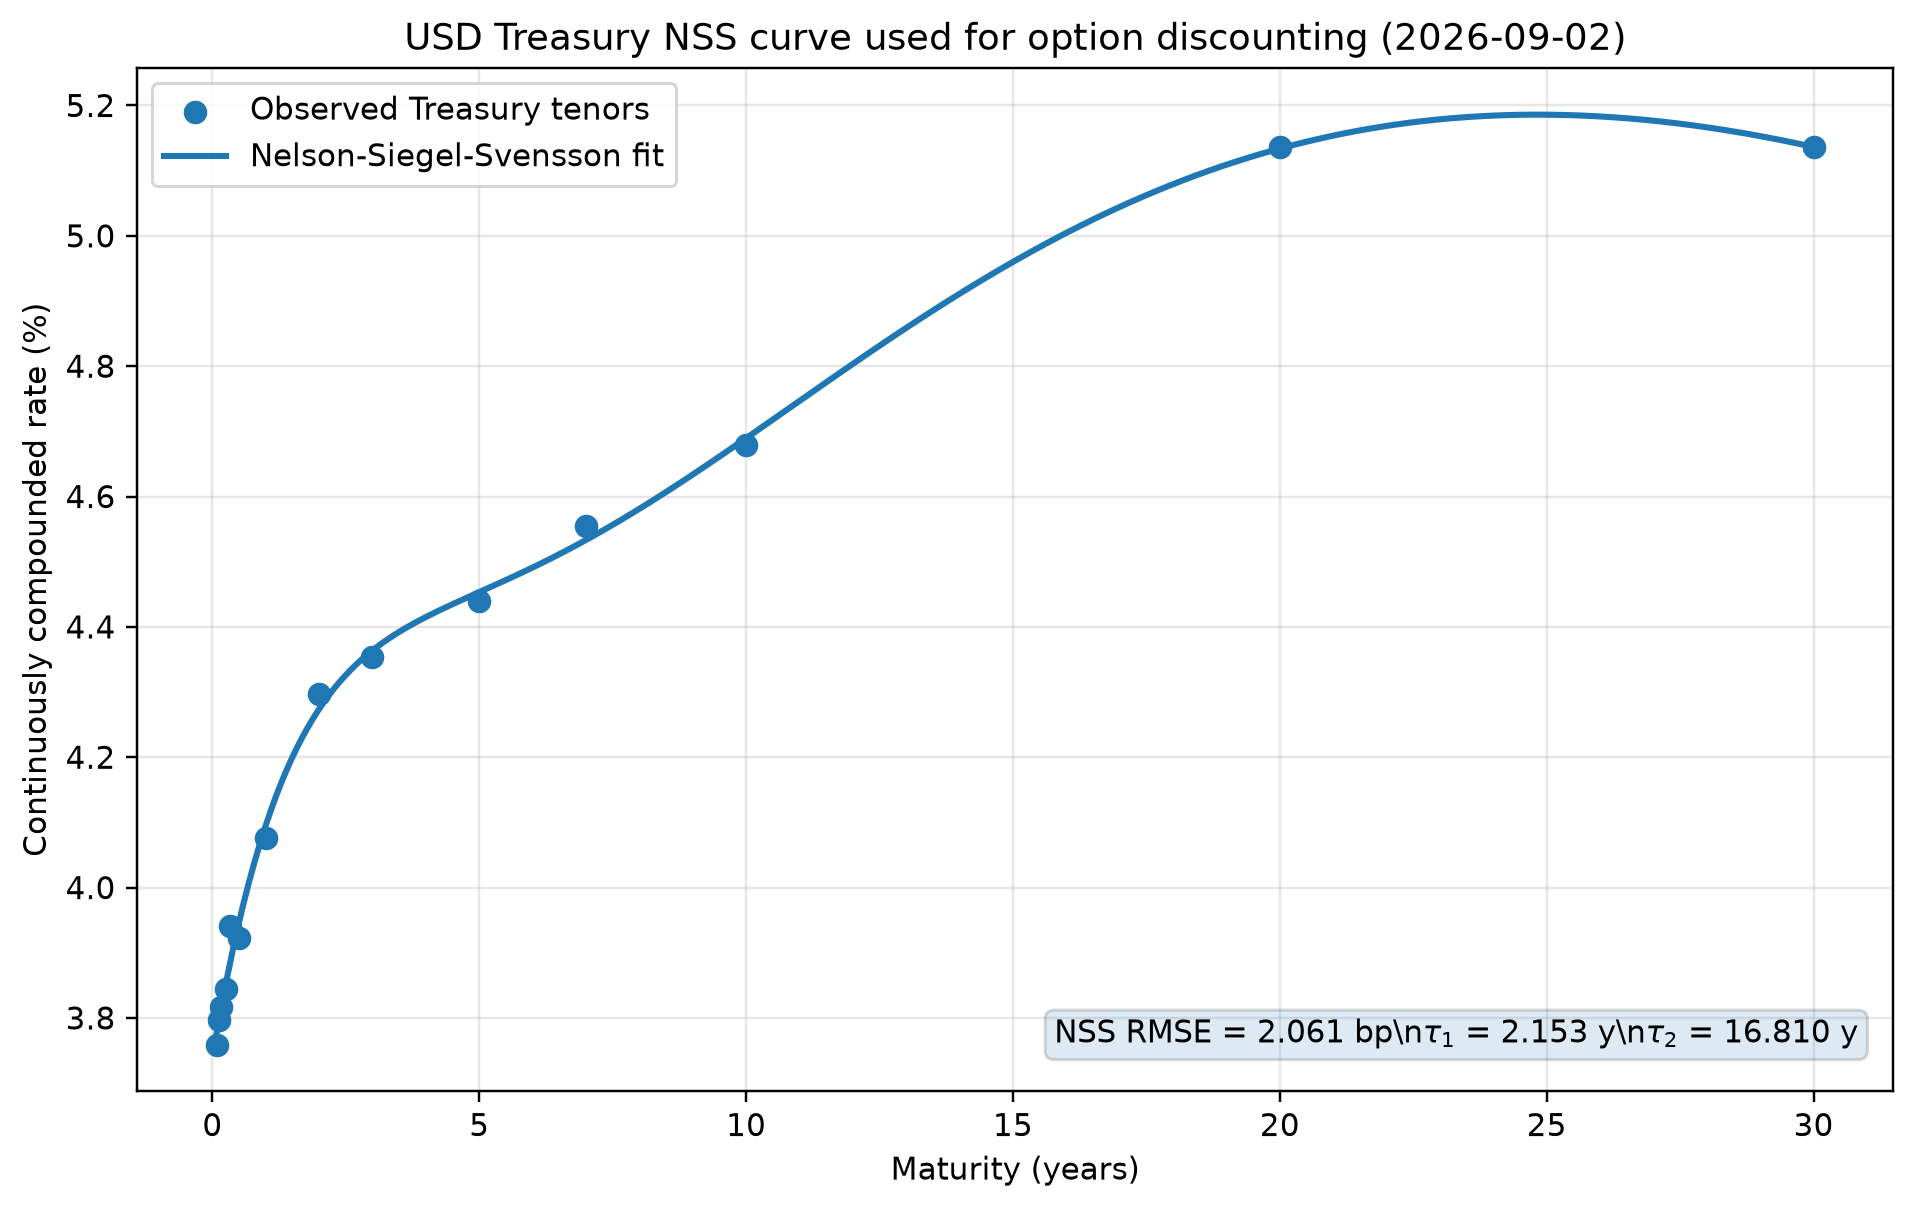
\includegraphics[width=0.82\textwidth]{img/team8_empirical/usd_treasury_curve.png}

    \vspace{4mm}
    
\includegraphics[width=0.88\textwidth]{img/team8_empirical/sampling_comparison.png}
    \caption{Team 8 calibration inputs. Top: 14 same-date continuously compounded U.S. Treasury proxies and their NSS fit
on 2 September 2026. Bottom: the CC64 sample selected from 605 eligible GLD calls
across 12 expiries and 146 strikes; the retained contracts span eight expiries
and 20 strikes. The colours encode observed
    implied volatility; the node layout, rather than an interpolated sheet,
    is the actual object passed to the optimizer.}
    \label{fig:t8-market-inputs}
\end{figure}

The historical GLD return series supplies a different diagnostic from the
option cross-section. It is observed under the historical data-generating
process and is used only to test Gaussian adequacy, not to estimate a physical
drift or to rank option-pricing models. Figure~\ref{fig:t8-return-normality}
shows both the central concentration and the tail departures that motivate a
variance-and-jump model stack.

\begin{figure}[H]
    \centering
    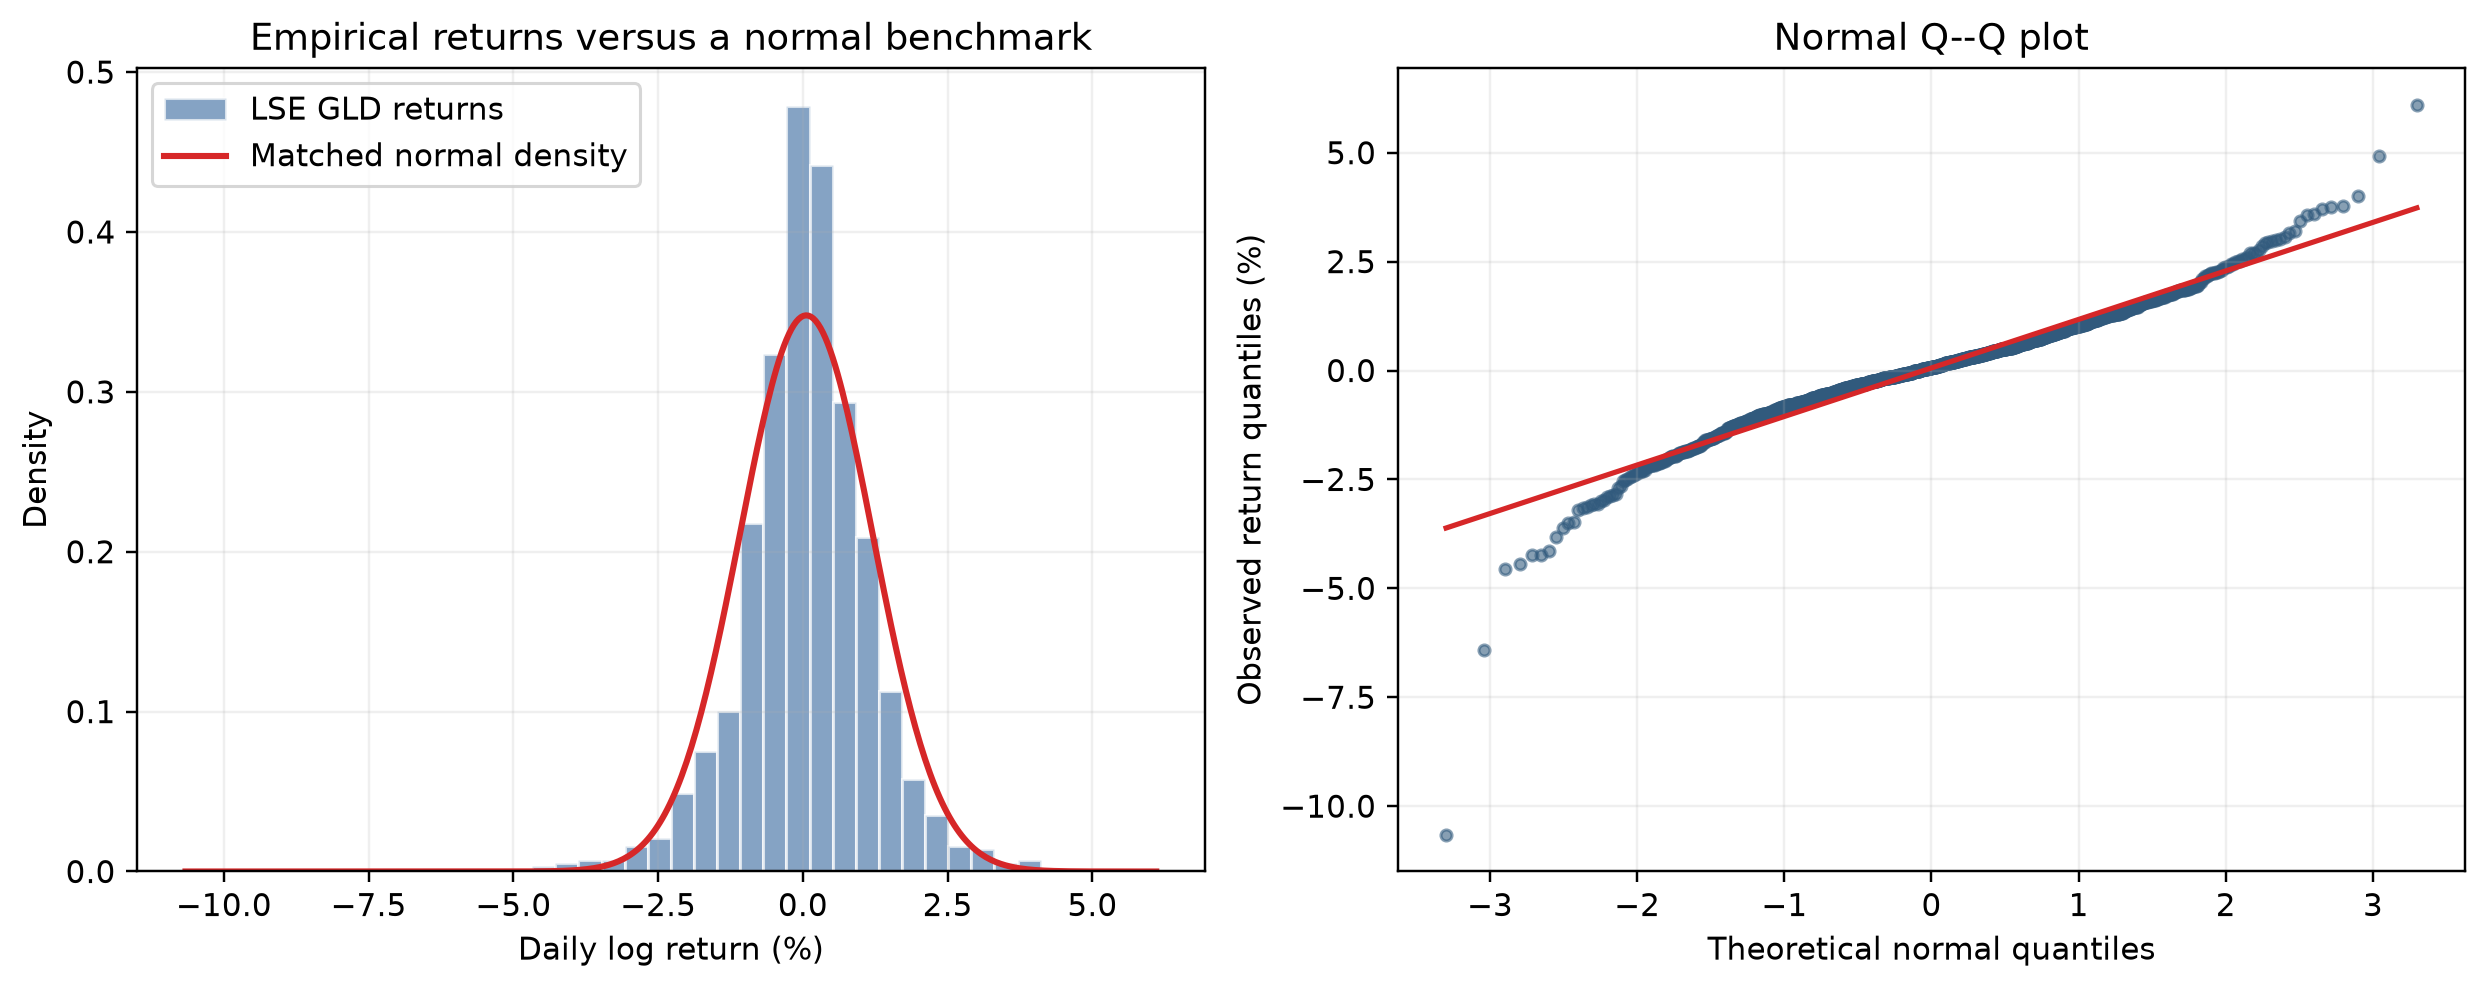
\includegraphics[width=0.96\textwidth]{img/team8_empirical/gld_return_normality.png}
    \caption{LSE GLD daily log returns from 5 January 2021 to 27 August 2026:
    empirical density against a matched normal law and normal Q--Q plot. The
    sample contains 1,424 observations; the visible tail departures are
    consistent with the formal tests in Table~\ref{tab:t8-return-normality}.}
    \label{fig:t8-return-normality}
\end{figure}

\begin{table}[H]
\centering
\footnotesize
\begin{tabular}{@{}lrrl@{}}
\toprule
Test & Statistic & \(p\)-value & Decision at 5\% \\
\midrule
Shapiro--Wilk & 0.9434 & \(6.25\cdot10^{-23}\) & Reject normality \\
Jarque--Bera & 3499.31 & \(<10^{-300}\) & Reject normality \\
D'Agostino \(K^2\) & 322.83 & \(7.90\cdot10^{-71}\) & Reject normality \\
\bottomrule
\end{tabular}
\caption{Normality tests for the 1,424 daily GLD log returns. Sample skewness
is \(-0.733\) and excess kurtosis is \(7.570\). Rejection motivates richer
dynamics but does not by itself select Heston, Bates or Bates--Hawkes.}
\label{tab:t8-return-normality}
\end{table}

\subsubsection{Cross-sectional calibration geometry}

Tables~\ref{tab:t8-model-parameters}--\ref{tab:t8-model-errors} consolidate
the point-in-time fit that is otherwise distributed across the model-specific
sections. All four rows use the same 64 actual nodes, price/IV conversion and
vega-weighted objective; richer models therefore change the state law rather
than the empirical target.

\begin{table}[H]
\centering
\scriptsize
\setlength{\tabcolsep}{2.6pt}
\begin{tabularx}{\textwidth}{@{}>{\RaggedRight\arraybackslash}p{2.35cm}>{\RaggedRight\arraybackslash}X>{\RaggedRight\arraybackslash}p{2.75cm}@{}}
\toprule
Model & Calibrated parameters & Admissibility \\
\midrule
Black--Scholes & \(\sigma=0.25088\). & Positive volatility. \\
Heston & \(v_0=0.06439,\; \kappa=4.05183,\; \theta_v=0.06548,\; \xi=0.72815,\; \rho=-0.01701\). & Feller gap 0.00043. \\
Bates--Poisson & \(v_0=0.06626,\; \kappa=4.05261,\; \theta_v=0.06324,\; \xi=0.67235,\; \rho=-0.03326,\; \lambda=0.24501,\; \mu_J=-0.02767,\; \sigma_J=0.00483\). & Feller gap 0.06053. \\
Full Bates--Hawkes & \(v_0=0.06514,\; \kappa=4.05259,\; \theta_v=0.06346,\; \xi=0.67263,\; \rho=-0.03322,\; \lambda_0=0.03496,\; \bar\lambda=0.56005,\; n=0.55690,\; \beta=2.74823,\; \mu_J=-0.02901,\; \sigma_J=0.02280\). & Feller gap 0.06196; stationary $n<1$. \\
\bottomrule
\end{tabularx}
\caption{Feller-constrained parameters on the current 2 September 2026 Team 8 Chebyshev sample.}
\label{tab:t8-model-parameters}
\end{table}

\begin{table}[H]
\centering
\scriptsize
\setlength{\tabcolsep}{3.1pt}
\begin{tabularx}{\textwidth}{@{}>{\RaggedRight\arraybackslash}p{2.35cm}rrrr>{\RaggedRight\arraybackslash}X@{}}
\toprule
Model & Price MAE & Price RMSE & IV MAE bp & IV RMSE bp & Reading \\
\midrule
Black--Scholes & 0.699 & 0.832 & 73.06 & 97.21 & Common CC64 target. \\
Heston & 0.398 & 0.501 & 38.48 & 49.49 & Lowest current in-sample error. \\
Bates--Poisson & 0.447 & 0.562 & 42.60 & 54.63 & Common CC64 target. \\
Full Bates--Hawkes & 0.410 & 0.514 & 40.76 & 52.97 & Common CC64 target. \\
\bottomrule
\end{tabularx}
\caption{Calibration errors on a common option sample. Heston has the lowest
in-sample IV RMSE; this cross-sectional fit is not an out-of-sample ranking.}
\label{tab:t8-model-errors}
\end{table}

The Full Bates--Hawkes branching ratio is 0.5569, below unity and away from
the former lower bound. This snapshot permits material self-excitation, but
does not establish stable identification across regimes. Heston remains the
current-fit winner; Hawkes is selected separately on rolling OOS performance.

The residual maps in Figures~\ref{fig:t8-residual-atlas-diffusion} and
\ref{fig:t8-residual-atlas-jumps} restore the spatial information hidden by
one RMSE. The continuous colours are interpolation only inside the observed
node domain; the circles identify the observations. Their purpose is to show
where errors remain systematic across maturity and moneyness.

\begin{figure}[p]
    \centering
    
\includegraphics[width=0.49\textwidth]{img/team8_empirical/black_scholes_residual_heatmap.png}\hfill
    
\includegraphics[width=0.49\textwidth]{img/team8_empirical/heston_residual_heatmap.png}
    \caption{Market-minus-model implied-volatility residuals for the two
    diffusion specifications: Black--Scholes (left) and Feller-constrained
    Heston (right). Stochastic variance reduces the scalar loss but does not
    remove structured maturity--moneyness error.}
    \label{fig:t8-residual-atlas-diffusion}
\end{figure}

\begin{figure}[p]
    \centering
    
\includegraphics[width=0.49\textwidth]{img/team8_empirical/bates_residual_heatmap.png}\hfill
    
\includegraphics[width=0.49\textwidth]{img/team8_empirical/bates_hawkes_residual_heatmap.png}
    \caption{Market-minus-model implied-volatility residuals after adding
    discontinuities: Bates--Poisson (left) and Full Bates--Hawkes (right).
    The Hawkes layer lowers the current scalar error, while visible clusters
    remain and residual normality is still rejected.}
    \label{fig:t8-residual-atlas-jumps}
\end{figure}

\begin{figure}[p]
    \centering
    
\includegraphics[width=0.97\textwidth]{img/team8_empirical/bates_hawkes_volatility_smile.png}
    \caption{Observed and Full Bates--Hawkes implied-volatility smiles across
    the eight sampled expiries. The panel view prevents a low aggregate RMSE
    from concealing expiry-specific misses, especially at boundary strikes.}
    \label{fig:t8-bh-smiles}
\end{figure}

The standalone study also compared three Hawkes routes that estimate
different objects. Table~\ref{tab:t8-hawkes-routes} preserves that distinction:
event-time likelihoods are kernel diagnostics, whereas only an option-price
calibration can enter the like-for-like surface comparison.

\begin{table}[H]
\centering
\scriptsize
\setlength{\tabcolsep}{3pt}
\begin{tabularx}{\textwidth}{@{}p{2.25cm}p{2.55cm}p{3.45cm}X@{}}
\toprule
Route & Target & Frozen result & Role \\
\midrule
Exact constant-volatility Hawkes & GLD option surface & \(\sigma=0.22448\),
\(n=0.00460\), objective \(8.674\cdot10^{-5}\). & Transform benchmark;
excludes the Heston variance state. \\
Exponential kernel & Event times & \(n=0.3884\), log-likelihood \(-67.75\),
AIC 141.51, BIC 147.36. & Stable Markovian kernel compatible with affine
pricing. \\
Rough power-law kernel & Event times & \(n=0.4119\), log-likelihood \(-68.03\),
AIC 144.05, BIC 151.86. & Long-memory diagnostic; not the option-pricing
model used in the comparison. \\
\bottomrule
\end{tabularx}
\caption{Historical source-study Hawkes routes; these frozen estimates are not the current September parameter set.}
\label{tab:t8-hawkes-routes}
\end{table}

\begin{figure}[p]
    \centering
    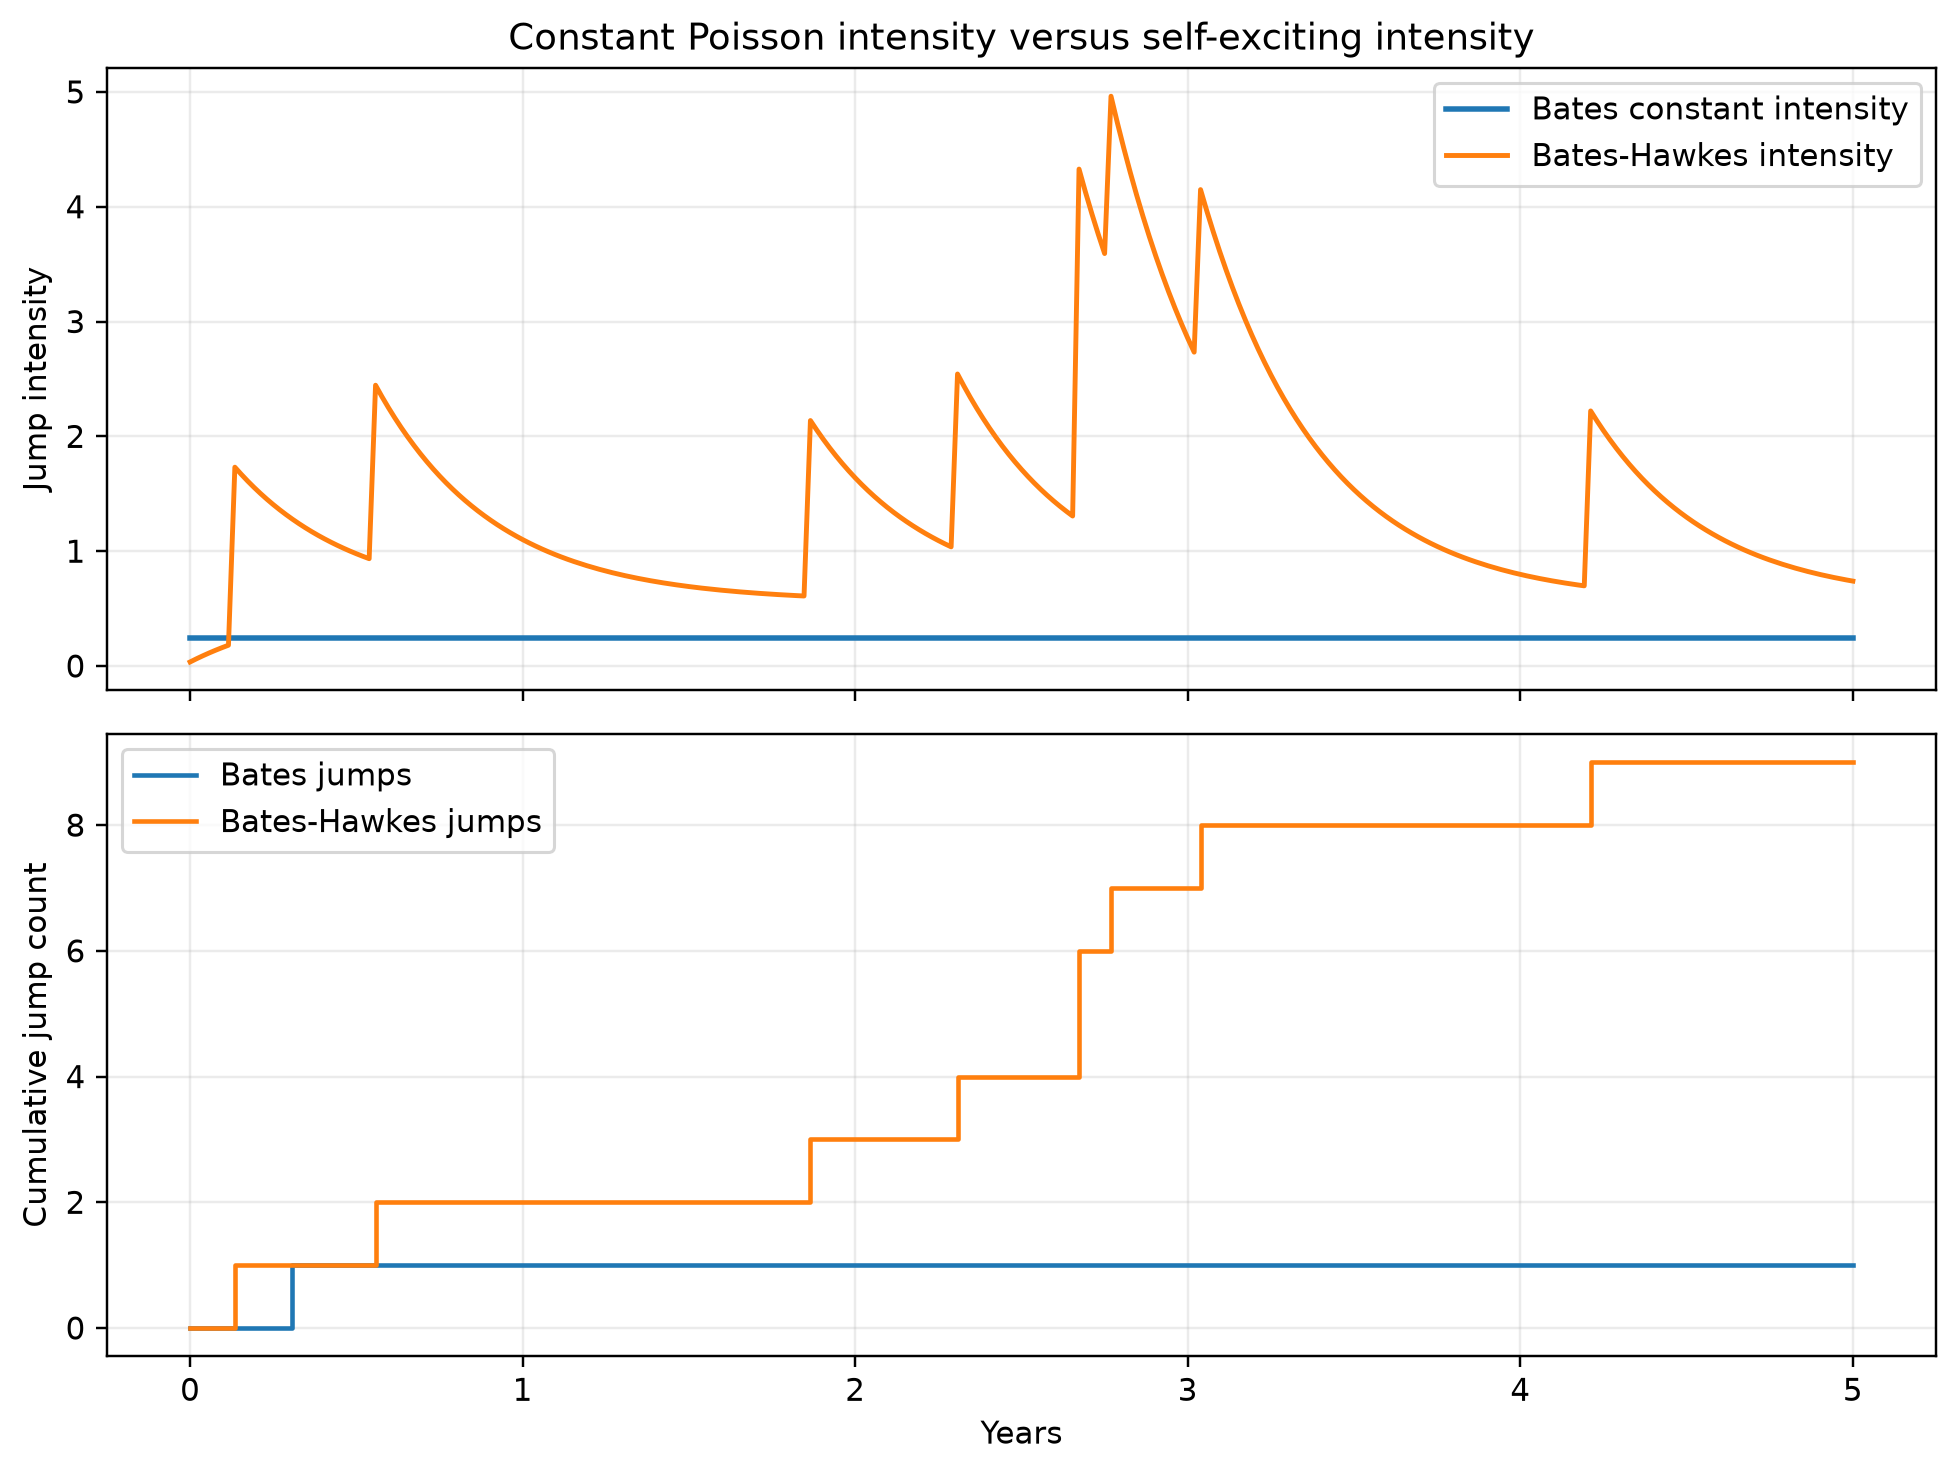
\includegraphics[width=0.94\textwidth]{img/team8_empirical/hawkes_intensity_comparison.png}
    \caption{Constant-intensity Bates jumps versus self-exciting
    Bates--Hawkes jumps regenerated from the current calibration. A Hawkes arrival raises
    near-term intensity, which subsequently decays toward its baseline; the
    lower panel shows the associated clustered event counts.}
    \label{fig:t8-hawkes-intensity}
\end{figure}

\begin{figure}[p]
    \centering
    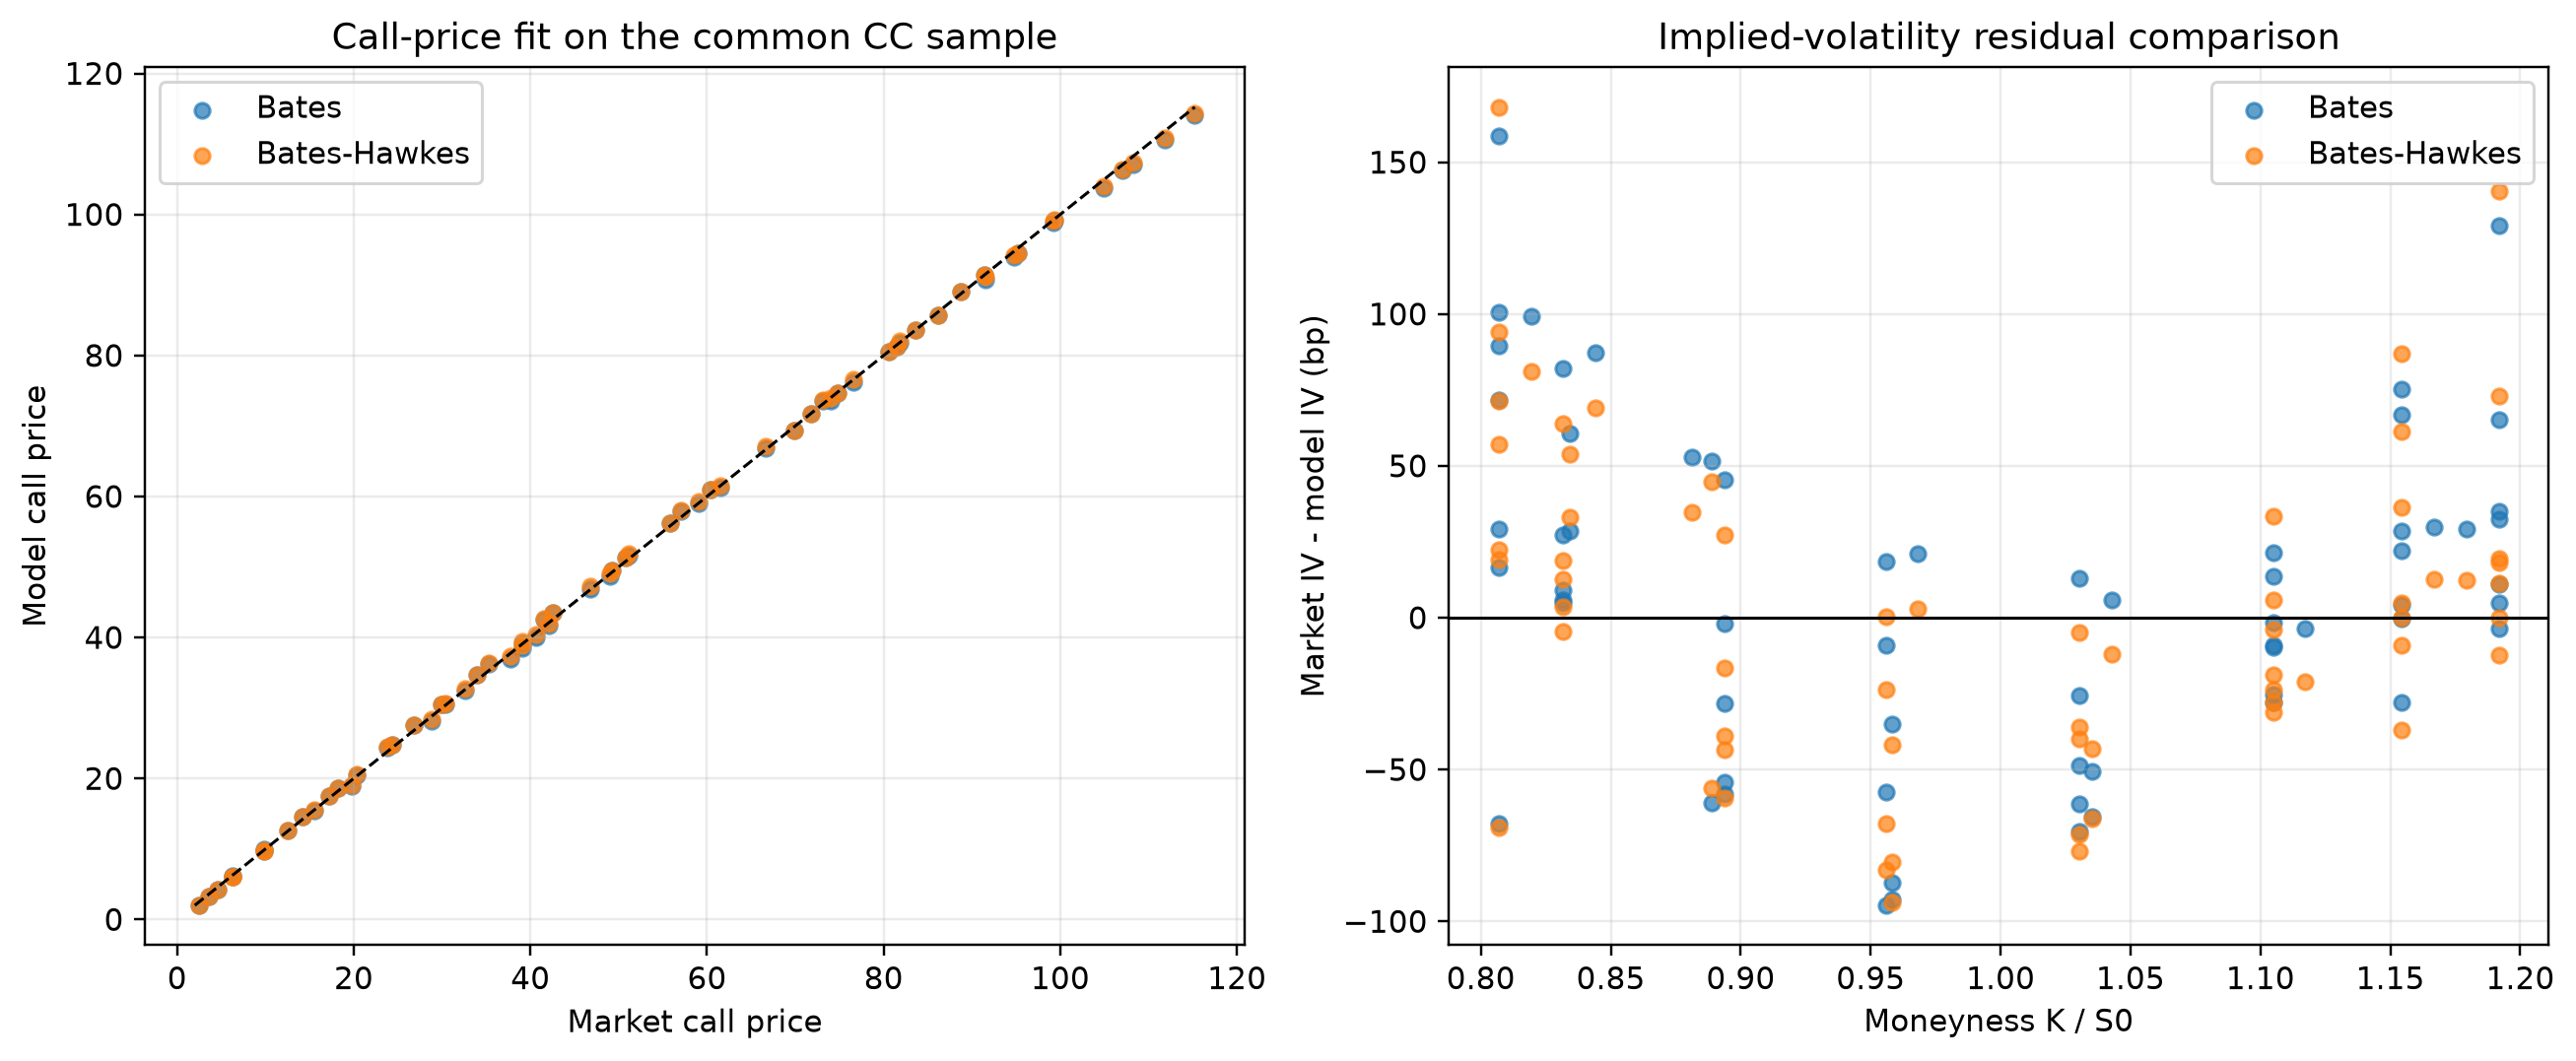
\includegraphics[width=0.98\textwidth]{img/team8_empirical/bates_hawkes_vs_bates.png}
    \caption{Direct current-snapshot comparison between Full Bates--Hawkes and
    Bates--Poisson. The left panel checks option prices against the diagonal;
    the right panel compares market-minus-model IV residuals by maturity. This
    is cross-sectional fit evidence, not proof of predictive dominance.}
    \label{fig:t8-bh-versus-bates}
\end{figure}

\subsubsection{Chronological loss accumulation}

Figure~\ref{fig:t8-welch-goyal} displays the September dense-only rolling
loss differences. The benchmark is the origin cross-sectional mean IV or the
interpolated origin IV surface. Black--Scholes does not beat the mean benchmark;
the three richer models do, but none beats persistence. Full Bates--Hawkes has
the lowest date-equal IV RMSE among the four candidates. These benchmark
comparisons do not establish physical gold forecasting accuracy.

\begin{figure}[p]
    \centering
    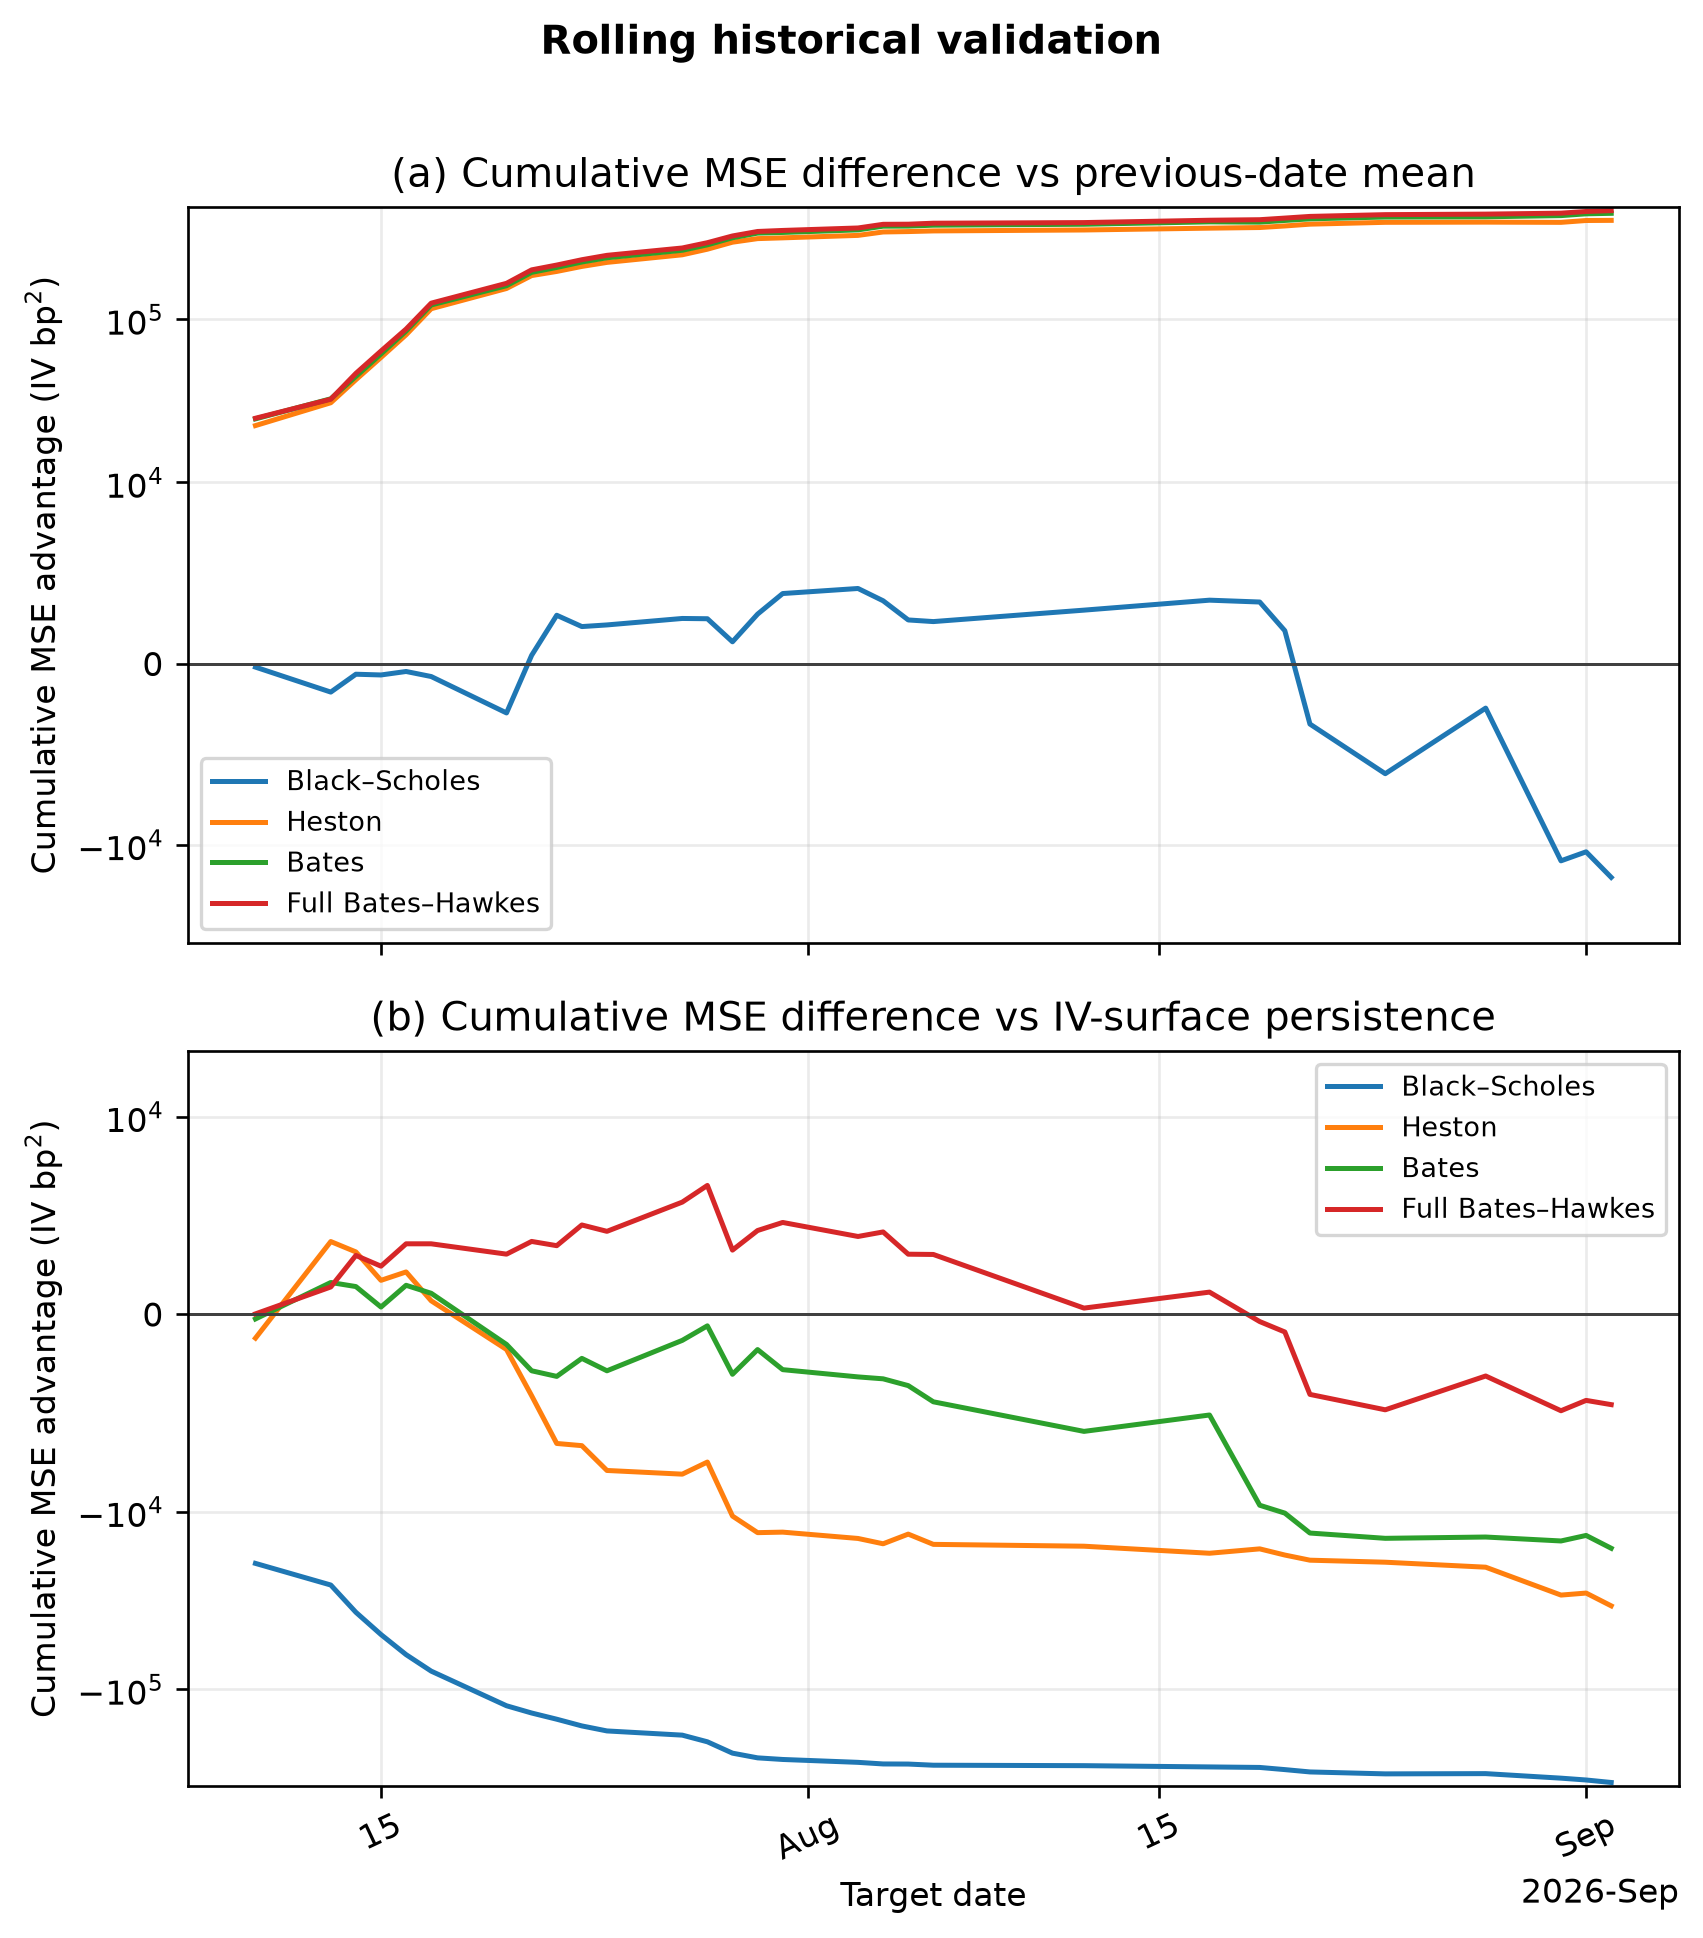
\includegraphics[width=0.98\textwidth]{img/team8_empirical/online_welch_goyal_cumulative.png}
    \caption{Dense-only rolling one-step-ahead Welch--Goyal cumulative squared-error
    differences over the Team 8 validation window, freshly rendered from
    aggregate outputs. Upward movement favours
    the named model relative to the comparator in each panel. The time path
    explains why a positive comparison with the origin mean coexists with
    failure against yesterday's observed IV surface.}
    \label{fig:t8-welch-goyal}
\end{figure}
